\documentclass[12pt,]{krantz}
\usepackage{lmodern}
\usepackage{amssymb,amsmath}
\usepackage{ifxetex,ifluatex}
\usepackage{fixltx2e} % provides \textsubscript
\ifnum 0\ifxetex 1\fi\ifluatex 1\fi=0 % if pdftex
  \usepackage[T1]{fontenc}
  \usepackage[utf8]{inputenc}
\else % if luatex or xelatex
  \ifxetex
    \usepackage{mathspec}
  \else
    \usepackage{fontspec}
  \fi
  \defaultfontfeatures{Ligatures=TeX,Scale=MatchLowercase}
    \setmonofont[Mapping=tex-ansi,Scale=0.7]{Source Code Pro}
\fi
% use upquote if available, for straight quotes in verbatim environments
\IfFileExists{upquote.sty}{\usepackage{upquote}}{}
% use microtype if available
\IfFileExists{microtype.sty}{%
\usepackage{microtype}
\UseMicrotypeSet[protrusion]{basicmath} % disable protrusion for tt fonts
}{}
\usepackage[unicode=true]{hyperref}
\PassOptionsToPackage{usenames,dvipsnames}{color} % color is loaded by hyperref
\hypersetup{
            pdftitle={Introduction to Data Science},
            pdfauthor={Hui Lin and Ming Li},
            colorlinks=true,
            linkcolor=Maroon,
            citecolor=Blue,
            urlcolor=Blue,
            breaklinks=true}
\urlstyle{same}  % don't use monospace font for urls
\usepackage{natbib}
\bibliographystyle{apalike}
\usepackage{longtable,booktabs}
\usepackage{graphicx,grffile}
\makeatletter
\def\maxwidth{\ifdim\Gin@nat@width>\linewidth\linewidth\else\Gin@nat@width\fi}
\def\maxheight{\ifdim\Gin@nat@height>\textheight\textheight\else\Gin@nat@height\fi}
\makeatother
% Scale images if necessary, so that they will not overflow the page
% margins by default, and it is still possible to overwrite the defaults
% using explicit options in \includegraphics[width, height, ...]{}
\setkeys{Gin}{width=\maxwidth,height=\maxheight,keepaspectratio}
\IfFileExists{parskip.sty}{%
\usepackage{parskip}
}{% else
\setlength{\parindent}{0pt}
\setlength{\parskip}{6pt plus 2pt minus 1pt}
}
\setlength{\emergencystretch}{3em}  % prevent overfull lines
\providecommand{\tightlist}{%
  \setlength{\itemsep}{0pt}\setlength{\parskip}{0pt}}
\setcounter{secnumdepth}{5}
% Redefines (sub)paragraphs to behave more like sections
\ifx\paragraph\undefined\else
\let\oldparagraph\paragraph
\renewcommand{\paragraph}[1]{\oldparagraph{#1}\mbox{}}
\fi
\ifx\subparagraph\undefined\else
\let\oldsubparagraph\subparagraph
\renewcommand{\subparagraph}[1]{\oldsubparagraph{#1}\mbox{}}
\fi
\usepackage{booktabs}
\usepackage{longtable}
\usepackage[bf,singlelinecheck=off]{caption}

\setmainfont[UprightFeatures={SmallCapsFont=AlegreyaSC-Regular}]{Alegreya}

\usepackage{framed,color}
\definecolor{shadecolor}{RGB}{248,248,248}

\renewcommand{\textfraction}{0.05}
\renewcommand{\topfraction}{0.8}
\renewcommand{\bottomfraction}{0.8}
\renewcommand{\floatpagefraction}{0.75}

\renewenvironment{quote}{\begin{VF}}{\end{VF}}
\let\oldhref\href
\renewcommand{\href}[2]{#2\footnote{\url{#1}}}

\ifxetex
  \usepackage{letltxmacro}
  \setlength{\XeTeXLinkMargin}{1pt}
  \LetLtxMacro\SavedIncludeGraphics\includegraphics
  \def\includegraphics#1#{% #1 catches optional stuff (star/opt. arg.)
    \IncludeGraphicsAux{#1}%
  }%
  \newcommand*{\IncludeGraphicsAux}[2]{%
    \XeTeXLinkBox{%
      \SavedIncludeGraphics#1{#2}%
    }%
  }%
\fi

\makeatletter
\newenvironment{kframe}{%
\medskip{}
\setlength{\fboxsep}{.8em}
 \def\at@end@of@kframe{}%
 \ifinner\ifhmode%
  \def\at@end@of@kframe{\end{minipage}}%
  \begin{minipage}{\columnwidth}%
 \fi\fi%
 \def\FrameCommand##1{\hskip\@totalleftmargin \hskip-\fboxsep
 \colorbox{shadecolor}{##1}\hskip-\fboxsep
     % There is no \\@totalrightmargin, so:
     \hskip-\linewidth \hskip-\@totalleftmargin \hskip\columnwidth}%
 \MakeFramed {\advance\hsize-\width
   \@totalleftmargin\z@ \linewidth\hsize
   \@setminipage}}%
 {\par\unskip\endMakeFramed%
 \at@end@of@kframe}
\makeatother

% \renewenvironment{Shaded}{\begin{kframe}}{\end{kframe}}

\newenvironment{rmdblock}[1]
  {
  \begin{itemize}
  \renewcommand{\labelitemi}{
    \raisebox{-.7\height}[0pt][0pt]{
      {\setkeys{Gin}{width=3em,keepaspectratio}\includegraphics{images/#1}}
    }
  }
  \setlength{\fboxsep}{1em}
  \begin{kframe}
  \item
  }
  {
  \end{kframe}
  \end{itemize}
  }
\newenvironment{rmdnote}
  {\begin{rmdblock}{note}}
  {\end{rmdblock}}
\newenvironment{rmdcaution}
  {\begin{rmdblock}{caution}}
  {\end{rmdblock}}
\newenvironment{rmdimportant}
  {\begin{rmdblock}{important}}
  {\end{rmdblock}}
\newenvironment{rmdtip}
  {\begin{rmdblock}{tip}}
  {\end{rmdblock}}
\newenvironment{rmdwarning}
  {\begin{rmdblock}{warning}}
  {\end{rmdblock}}

\usepackage{makeidx}
\makeindex

\urlstyle{tt}

\usepackage{amsthm}
\makeatletter
\def\thm@space@setup{%
  \thm@preskip=8pt plus 2pt minus 4pt
  \thm@postskip=\thm@preskip
}
\makeatother

\frontmatter

\title{Introduction to Data Science}
\author{\href{http://scientistcafe.com}{Hui Lin} and Ming Li}
\date{2017-12-05}

\usepackage{amsthm}
\newtheorem{theorem}{Theorem}[section]
\newtheorem{lemma}{Lemma}[section]
\theoremstyle{definition}
\newtheorem{definition}{Definition}[section]
\newtheorem{corollary}{Corollary}[section]
\newtheorem{proposition}{Proposition}[section]
\theoremstyle{definition}
\newtheorem{example}{Example}[section]
\theoremstyle{remark}
\newtheorem*{remark}{Remark}
\begin{document}
\maketitle

%\cleardoublepage\newpage\thispagestyle{empty}\null
%\cleardoublepage\newpage\thispagestyle{empty}\null
%\cleardoublepage\newpage
\thispagestyle{empty}
\begin{center}
%\includegraphics{images/dedication.pdf}
\end{center}

\setlength{\abovedisplayskip}{-5pt}
\setlength{\abovedisplayshortskip}{-5pt}

{
\hypersetup{linkcolor=black}
\setcounter{tocdepth}{3}
\tableofcontents
}
\listoftables
\listoffigures
\section*{Copyright Statement}\label{copyright-statement}


Please note that this work is being written under a
\href{https://github.com/happyrabbit/IntroDataScience/blob/master/CONDUCT.md}{Contributor
Code of Conduct} and released under a
\href{https://creativecommons.org/licenses/by-nc-sa/3.0/us/}{CC-BY-NC-SA
license}. By participating in this project (for example, by submitting a
\href{https://github.com/happyrabbit/IntroDataScience/issues}{pull
request} with suggestions or edits) you agree to abide by its terms.

A hard copy will be published by CRC Press. The expected date is Dec 1,
2019.

\section*{About the Authors}\label{about-the-authors}


\textbf{Hui Lin} is currently Data Scientist at DuPont Pioneer. She is a
leader within DuPont at applying advanced data science to enhance
Marketing and Sales effectiveness. She has been providing statistical
leadership for a broad range of predictive analytics and market research
analysis since 2013. She is the co-founder of Central Iowa R User Group,
blogger of scientistcafe.com and program Chair of Statistics in
Marketing Section of ASA for 2018. She enjoys making analytics
accessible to a broad audience and teaches tutorials and workshops for
practitioners on data science.

She holds MS and Ph.D.~in statistics from Iowa State University, BS in
mathematical statistics from Beijing Normal University.

\textbf{Ming Li} is currently a Sr. Data Scientist at Amazon. He was
Data Scientist at Wal-Mart and an Adjunct Faculty of Department and
Marketing and Business Analytics in TAMU -- Commerce. He is also the
Chair of Quality \& Productivity Section of ASA for 2016. He was a
Statistical Leader at General Electric Global Research Center and
Research Statistician at SAS Institute. He obtained his Ph.D.~in
Statistics from Iowa State University at 2010. With deep statistics
background and a few years' experience in data science, he has trained
and mentored numerous junior data scientist with different backgrounds
such as statistics, computer science, and business analytics.

\section*{Acknowledgements}\label{acknowledgements}


We want to give special thanks to Alex Shum and David Body for their
editing and comments on the sections of this book.

\section{Introduction}\label{introduction}

Interest in data science is at an all time high and really has exploded
in popularity in the last couple of years. Data scientists today are
from various backgrounds. If someone ran into you asked what data
science was all about, what would you tell them?

Various professional statistics organizations are reacting to this
confusing situation. (Page 5-7, ``50 Years of Data Science'') From those
discussions, Donoho summarizes the main recurring ``Memes'' about data
sciences:

\begin{enumerate}
\def\labelenumi{\arabic{enumi}.}
\tightlist
\item
  The `Big Data' Meme
\item
  The `Skills' Meme
\item
  The `Jobs' Meme
\end{enumerate}

Everyone should have heard about big data. The media hasn't taken a
minute break from touting ``big'' data. Data science trainees now need
the skills to cope with such big data sets. What are those skills? You
may hear about: Hadoop, system using Map/Reduce to process large data
sets distributed across a cluster of computers. The new skills are for
dealing with organizational artifacts of large-scale cluster computing
but not for better solving the real problem. A lot of data on its own is
worthless. It isn't the size of the data that's important. It's what you
do with it. The big data skills that so many are touting today are not
skills for better solving the real problem of inference from data.

We are transiting to universal connectivity with a deluge of data
filling telecom servers. But these facts don't immediately create a
science. The statisticians and computer scientists have been laying the
groundwork of data science for at least 50 years. Today's data science
is an enlargement and combination of statistics and computer science
rather than a brand new discipline.

\subsection{What is data science?}\label{what-is-data-science}

Data Science doesn't come out of the blue. Its predecessor is data
analysis. Back in 1962, John Tukey wrote in ``The Future of Data
Analysis'':

\begin{quote}
For a long time I have thought I was a statistician, interested in
inferences from the particular to the general. But as I have watched
mathematical statistics evolve, I have had cause to wonder and to doubt.
\ldots{}All in all, I have come to feel that my central interest is in
data analysis, which I take to include, among other things: procedures
for analyzing data, techniques for interpreting the results of such
procedures, ways of planning the gathering of data to make its analysis
easier, more precise or more accurate, and all the machinery and results
of (mathematical) statistics which apply to analyzing data.
\end{quote}

It deeply shocked his academic readers. Aren't you supposed to present
something mathematically precise, such as definitions, theorems and
proofs? If we use one sentence to summarize what John said, it is:

\begin{quote}
data analysis is more than mathematics.
\end{quote}

In September 2015, the University of Michigan make plans to invest \$100
million over the next five years in a new
\href{http://www.ns.umich.edu/new/releases/23105-u-michigan-launches-100-million-data-science-initiative}{Data
Science Initiative} that will enhance opportunities for student and
faculty researchers across the university to tap into the enormous
potential of big data. UM Provost Martha Pollack said:

\begin{quote}
``Data science has become a fourth approach to scientific discovery, in
addition to experimentation, modeling and computation,\ldots{}''
\end{quote}

How does the Data Science Initiative define Data science? Their website
gives us an idea:

\begin{quote}
``This coupling of scientific discovery and practice involves the
collection, management, processing, analysis, visualization, and
interpretation of vast amounts of heterogeneous data associated with a
diverse array of scientific, translational, and interdisciplinary
applications.''
\end{quote}

With the data science hype picking up stream, many professionals changed
their titles to Data Scientist without any of the necessary
qualifications. But at that time, the data scientist title was not well
defined which lead to confusion in the market, obfuscation in resumes,
and exaggeration of skills. Here is a list of somewhat whimsical
definitions for a ``data scientist'':

\begin{itemize}
\tightlist
\item
  ``A data scientist is a data analyst who lives in California''
\item
  ``A data scientist is someone who is better at statistics than any
  software engineer and better at software engineering than any
  statistician.''
\item
  ``A data scientist is a statistician who lives in San Francisco.''
\item
  ``Data Science is statistics on a Mac.''
\end{itemize}

There is lots of confusion between Data Scientist, Statistician,
Business/Financial/Risk(etc) Analyst and BI professional due to the
obvious intersections among skillsets. We see data science as a
discipline to make sense of data. In order to make sense of data,
statistics is indispensable. But a data scientist also needs many other
skills.

In the obscenity case of Jacobellis v. Ohio (1964), Potter Stewart wrote
in his short concurrence that ``hard-core pornography'' was hard to
define, but that ``I know it when I see it.'' This applies to many
things including data science. It is hard to define but you know it when
you see it.

So instead of scratching my head to figure out a one sentence
definition, we are going to sketch the history of data science, what
kind of questions data science can answer, and describe the skills
required for being a data scientist. We hope this can give you a better
depiction of data science.

In the early 19th century when Legendre and Gauss came up the least
squares method for linear regression, only physicists would use it to
fit linear regression. Now, even non-technical people can fit linear
regressions using excel. In 1936 Fisher came up with linear discriminant
analysis. In the 1940s, we had another widely used model -- logistic
regression. In the 1970s, Nelder and Wedderburn formulated ``generalized
linear model (GLM)'' which:

\begin{quote}
``generalized linear regression by allowing the linear model to be
related to the response variable via a link function and by allowing the
magnitude of the variance of each measurement to be a function of its
predicted value.'' {[}from Wikipedia{]}
\end{quote}

By the end of the 1970s, there was a range of analytical models and most
of them were linear because computers were not powerful enough to fit
non-linear model until the 1980s.

In 1984 Breiman et al. introduced classification and regression tree
(CART) which is one of the oldest and most utilized classification and
regression techniques. After that Ross Quinlan came up with more tree
algorithms such as ID3, C4.5 and C5.0. In the 1990s, ensemble techniques
(methods that combine many models' predictions) began to appear. Bagging
is a general approach that uses bootstrapping in conjunction with any
regression or classification model to construct an ensemble. Based on
the ensemble idea, Breiman came up with random forest in 2001. Later,
Yoav Freund and Robert Schapire came up with the AdaBoost.M1 algorithm.
Benefiting from the increasing availability of digitized information,
and the possibility to distribute that via the internet, the tool box
has been expanding fast. The applications include business, health,
biology, social science, politics etc.

John Tukey identified 4 forces driving data analysis (there was no
``data science'' then):

\begin{enumerate}
\def\labelenumi{\arabic{enumi}.}
\tightlist
\item
  The formal theories of math and statistics
\item
  Acceleration of developments in computers and display devices
\item
  The challenge, in many fields, of more and ever larger bodies of data
\item
  The emphasis on quantification in an ever wider variety of disciplines
\end{enumerate}

Tukey's 1962 list is surprisingly modern. Let's inspect those points in
today's context. There is always a time gap between a theory and its
application. We had the theories much earlier than application.
Fortunately, for the past 50 years statisticians have been laying the
theoretical groundwork for constructing ``data science'' today. The
development of computers enables us to calculate much faster and deliver
results in a friendly and intuitive way. The striking transition to the
internet of things generates vast amounts of commercial data. Industries
have also sensed the value of exploiting that data. Data science seems
certain to be a major preoccupation of commercial life in coming
decades. All the four forces John identified exist today and have been
driving data science.

\subsection{Is it science? Totally?}\label{is-it-science-totally}

Let's take one step back. What is science? Here is what John Tukey said:

\begin{quote}
There are diverse views as to what makes a science, but three
constituents will be judged essential by most, viz:\\
(a1) intellectual content,\\
(a2) organization in an understandable form,\\
(a3) reliance upon the test of experience as the ultimate standard of
validity
\end{quote}

The first one (a1) doesn't provide useful information. And (a2) can't
distinguish science from art very well. The last one is a key character
of science. The influential philosopher of science Karl Popper argued
that science advances by falsifying hypotheses. If science needs to be
falsifiable, then data science is not 100\% science. It is true that
there are some analytical results that can be validated (falsified)
through cross validation or comparing prediction with future outcomes.
But certainly not all of them. Even in the problem of prediction, we
can't validate predictions in the 2nd order chaotic systems.

We can't scientifically validate many unsupervised learning or
descriptive analysis, especially in the context of marketing. In that
sense, data science is a combination of science and art.\\
There is another definition of science from the famous computer
scientist Donald Knuth. He said in his legendary 1974 essay
\href{http://www.paulgraham.com/knuth.html}{Computer Programming as an
Art}:

\begin{quote}
``Science is knowledge which we understand so well that we can teach it
to a computer.''
\end{quote}

Computers are indispensable for data science. But can we teach computers
to do all the work data scientists do today? No. So it is not totally
science. Computers can't communicate with stakeholders to transform a
real life problem to be data problem. Computers don't know which
questions can be answered through analytics. Computers don't know how to
explain the results to different audiences using different ways
according to their backgrounds. Computers are powerful in many ways but
certainly not all. Would a computer enter a `runaway reaction' of
self-improvement cycles so that it could surpass human in every way in
the future? Well, that is not a question we are trying to answer here.
If you are interested in the future of technology, there are some books
you can refer to. Ray Kurzweil (The Singularity Is Near), Yuval Noah
Harari (Homo Deus: A Brief History of Tomorrow) and Kevin Kelly (The
Inevitable). At the risk of being short-sighted, we will assume it won't
happen in foreseeable future.

To be simple I will still use data science in the rest of the book. But
it is important to realize that data science includes art.

\subsection{What kind of questions can data science
solve?}\label{what-kind-of-questions-can-data-science-solve}

\subsubsection{Prerequisites}\label{prerequisites}

Data science is not a panacea, and data scientists are not magicians.
There are problems data science can't help. It is best to make a
judgment as early in the analytical cycle as possible. Tell your clients
honestly and clearly when you figure data analytics can't give the
answer they want. What kind of questions can data science solve? What
are the requirements for our question?

\begin{enumerate}
\def\labelenumi{\arabic{enumi}.}
\tightlist
\item
  Your question needs to be specific enough
\end{enumerate}

Look at two examples:

\begin{itemize}
\tightlist
\item
  Question 1: How can I increase product sales?
\item
  Question 2: Is the new promotional tool introduced at the beginning of
  this year boosting the annual sales of P1197 in Iowa and Wisconsin?
  (P1197 is an impressive corn seed product from DuPont Pioneer)
\end{itemize}

It is easy to see the difference between the two questions. Question 1
is a grammatically correct question, but it is proper for data analysis
to answer. Why? It is too general. What is the response variable here?
Product sales? Which product? Is it annual sales or monthly sales? What
are the candidate predictors? You nearly can't get any useful
information from the questions. In contrast, question 2 is much more
specific. From the analysis point of view, the response variable is
clearly ``annual sales of P1197 in Iowa and Wisconsin''. Even we don't
know all the predictors, but the variable of interest is ``the new
promotional tool introduced early this year.'' We want to study the
impact of the promotion on the sales. You can start from there and move
on to figure out other variables need to include in the model by further
communication.

As a data scientist, you may start with something general and unspecific
like question 1 and eventually get to question 2. Effective
communication and in-depth domain knowledge about the business problem
are essential to convert a general business question into a solvable
analytical problem. Domain knowledge helps data scientist communicate
with the language the other people can understand and obtain the
required information.

However, defining the question and variables involved don't guarantee
that you can answer it. I have encountered a well-defined supply chain
problem. My client asked about the stock needed for a product in a
particular area. Why can not this question be answered? I did fit a
Multivariate Adaptive Regression Spline (MARS) model and thought I found
a reasonable solution. But it turned out later that the data they gave
me was inaccurate. In some areas, only estimates of past supply figures
were available. The lesson lends itself to the next point.

\begin{enumerate}
\def\labelenumi{\arabic{enumi}.}
\setcounter{enumi}{1}
\tightlist
\item
  You need to have sound and relevant data
\end{enumerate}

One cannot make a silk purse out of a sow's ear. Data scientists need
data, sound and relevant data. The supply problem is a case in point.
There was relevant data, but not sound. All the later analytics based on
that data was a building on sand. Of course, data nearly almost have
noise, but it has to be in a certain range. Generally speaking, the
accuracy requirement for the independent variables of interest and
response variable is higher than others. In question 2, it is data
related to the ``new promotion'' and ``sales of P1197''.

The data has to be helpful for the question. If you want to predict
which product consumers are most likely to buy in the next three months,
you need to have historical purchasing data: the last buying time, the
amount of invoice, coupons and so on. Information about customers'
credit card number, ID number, the email address is not going to help.

Often the quality of the data is more important than the quantity, but
the quantity can not be overlooked. In the premise of guaranteeing
quality, usually the more data, the better. If you have a specific and
reasonable question, also sound and relevant data, then congratulations,
you can start playing data science!

\subsubsection{Problem type}\label{problem-type}

Many of the data science books classify the various models from a
technical point of view. Such as supervised vs.~unsupervised models,
linear vs.~nonlinear models, parametric models vs.~non-parametric
models, and so on. Here we will continue on ``problem-oriented'' track.
We first introduce different groups of real problems and then present
which models can be used to answer the corresponding category of
questions.

\begin{figure}[htbp]
\centering
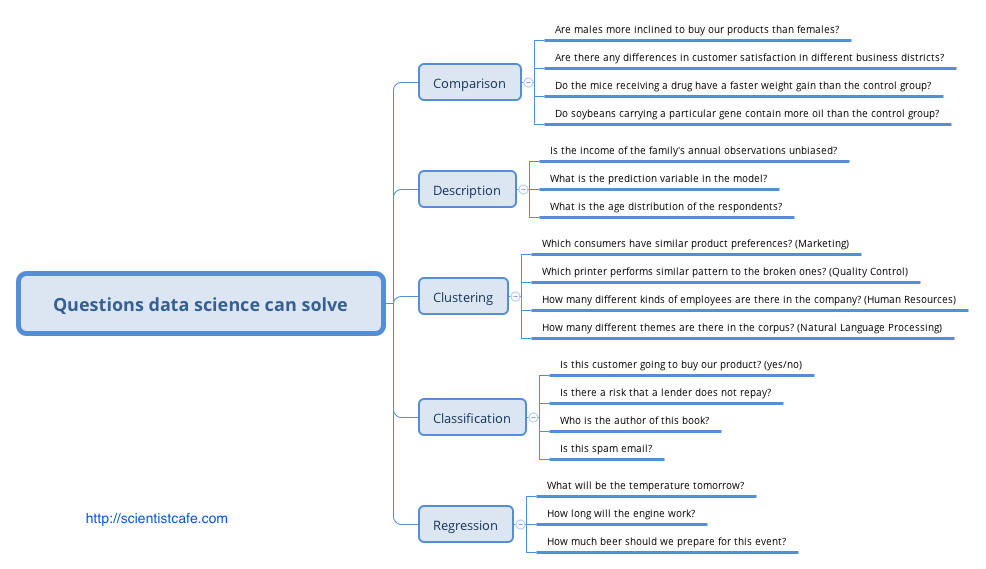
\includegraphics{images/DataScienceQuestion.png}
\caption{}
\end{figure}

\begin{enumerate}
\def\labelenumi{\arabic{enumi}.}
\tightlist
\item
  Comparison
\end{enumerate}

The first common problem is to compare different groups. Such as: Is A
better in some way than B? Or more comparisons: Is there any difference
among A, B, C in a certain aspect? Here are some examples:

\begin{itemize}
\tightlist
\item
  Are the purchasing amounts different between consumers receiving
  coupons and those without coupons?
\item
  Are males more inclined to buy our products than females?
\item
  Are there any differences in customer satisfaction in different
  business districts?
\item
  Do the mice receiving a drug have a faster weight gain than the
  control group?
\item
  Do soybeans carrying a particular gene contain more oil than the
  control group?
\end{itemize}

For those problems, it is usually to start exploring from the summary
statistics and visualization by groups. After a preliminary
visualization, you can test the differences between treatment and
control group statistically. The commonly used statistical tests are
chi-square test, t-test, and ANOVA. There are also methods using
Bayesian methods. In biology industry, such as new drug development,
crop breeding, mixed effect models are the dominant technique.

\begin{enumerate}
\def\labelenumi{\arabic{enumi}.}
\setcounter{enumi}{1}
\tightlist
\item
  Description
\end{enumerate}

In the problem such as customer segmentation, after you cluster the
sample, the next step is to figure out the profile of each class by
comparing the descriptive statistics of the various variables. Questions
of this kind are:

\begin{itemize}
\tightlist
\item
  Is the income of the family's annual observations unbiased?
\item
  What is the mean/variance of the monthly sales volume of a product in
  different regions?
\item
  What is the difference in the magnitude of the variable? (Decide
  whether the data needs to be standardized)
\item
  What is the prediction variable in the model?
\item
  What is the age distribution of the respondents?
\end{itemize}

Data description is often used to check data, find the appropriate data
preprocessing method, and demonstrate the model results.

\begin{enumerate}
\def\labelenumi{\arabic{enumi}.}
\setcounter{enumi}{2}
\tightlist
\item
  Clustering
\end{enumerate}

Clustering is a widespread problem, which is usually related to
classification. Clustering answers questions like:

\begin{itemize}
\tightlist
\item
  Which consumers have similar product preferences? (Marketing)
\item
  Which printer performs similar pattern to the broken ones? (Quality
  Control)
\item
  How many different kinds of employees are there in the company? (Human
  Resources)
\item
  How many different themes are there in the corpus? (Natural Language
  Processing)
\end{itemize}

Note that clustering is unsupervised learning. The most common
clustering algorithms include K-Means and Hierachical Clustering.

\begin{enumerate}
\def\labelenumi{\arabic{enumi}.}
\setcounter{enumi}{3}
\tightlist
\item
  Classification
\end{enumerate}

Usually, a labeled sample set is used as a training set to train the
classifier. Then the classifier is used to predict the category of a
future sample. Here are some example questions:

\begin{itemize}
\tightlist
\item
  Is this customer going to buy our product? (yes/no)
\item
  Is there a risk that a lender does not repay?
\item
  Who is the author of this book?
\item
  Is this spam email?
\end{itemize}

There are hundreds of classifiers. In practice, we do not have to try
all the models as long as we fit in several of the best models in most
cases.

\begin{enumerate}
\def\labelenumi{\arabic{enumi}.}
\setcounter{enumi}{4}
\tightlist
\item
  Regression
\end{enumerate}

In general, regression deals with the problem of ``how much is it?'' and
return a numerical answer. In some cases, it is necessary to coerce the
model results to be 0, or round the result to the nearest integer. It is
the most common problem.

\begin{itemize}
\tightlist
\item
  What will be the temperature tomorrow?
\item
  What will be the company's sales in the fourth quarter of this year?
\item
  How long will the engine work?
\item
  How much beer should we prepare for this event?
\end{itemize}

\subsection{What are the required skills for data
scientist?}\label{what-are-the-required-skills-for-data-scientist}

We talked about the bewildering definitions of data scientist. With the
data science hype picking up, some professionals have begun changing
their titles to Data Scientist without any of the necessary
qualifications (see
``\href{http://www.burtchworks.com/2013/06/12/data-scientists-or-data-wannabes/}{Data
Scientists\ldots{}or Data Wannabes}''). What are the required skills for
data scientist?

\begin{itemize}
\tightlist
\item
  Educational Background
\end{itemize}

Most of the data scientists today have undergraduate or higher degree
from one of the following areas: computer science, electronic
engineering, mathematics or statistics. According to a 2017 survey, 25\%
of US data scientists have a PhD degree, 64\% have a Master's degree,
and 11\% are Bachelors.

\begin{itemize}
\tightlist
\item
  Database Skills
\end{itemize}

Data scientists in the industry need to use SQL to pull data from the
database. So it is necessary to be familiar with how data is structured
and how to do basic data manipulation using SQL. Many
statistics/mathematics students do not have experience with SQL in
school. Don't worry. If you are proficient in one programming language,
it is easy to pick up SQL. The main purpose of graduate school should be
to develop the ability to learn and analytical thinking rather than the
technical skills. Even the technical skills are necessary to enter the
professional area. Most of the skills needed at work are not taught in
school.

\begin{itemize}
\tightlist
\item
  Programming Skills
\end{itemize}

Programming skills are critical for data scientists. According to a 2017
survey from
\href{http://www.burtchworks.com/2017/06/19/2017-sas-r-python-flash-survey-results/}{Burtch
Works}, 97\% of the data scientists today using R or Python. We will
focus on R in this book, but both are great tools for data science.
There is not one ``have-to-use'' tool. The goal is to solve the problem
not which tool to choose. However, a good tool needs to be flexible and
scalable.

\begin{itemize}
\tightlist
\item
  Modeling Skills
\end{itemize}

Data scientists need to know statistical and machine learning models.
There is no clear line separating these two. Many statistical models are
also machine learning models, vice versa. Generally speaking, a data
scientist is familiar with basic statistical tests such as t-test,
chi-square test, and analysis of variance. They can explain the
difference between Spearman rank correlation and Pearson correlation, be
aware of basic sampling schemes, such as Simple Random Sampling,
Stratified Random Sampling, and Multi-Stage Sampling. Know commonly used
probability distributions such as Normal distribution, Binomial
distribution, Poisson distribution, F distribution, T distribution, and
Chi-square distribution. Experimental design plays a significant role in
the biological study. Understanding the main tenants of Bayesian methods
is necessary (at least be able to write the Bayes theorem on the
whiteboard and know what does it mean). Know the difference between
supervised and unsupervised learning. Understand commonly used cluster
algorithms, classifiers, and regression models. Some powerful tools in
predictive analytics are tree models (such as random forest and
AdaBoost) and penalized model (such as lasso and SVM). Data scientist
working on social science (such as consumer awareness surveys), also
needs to know the latent variable model, such as exploratory factor
analysis, confirmatory factor analysis, structural equation model.

Is the list getting a little scary? It can get even longer. Don't worry
if you don't know all of them now. You will learn as you go. Standard
mathematics, statistics or computer science training in graduate school
can get you started. But you have to learn lots of new skills after
school. Learning is happening increasingly outside of formal educational
settings and in unsupervised environments. An excellent data scientist
must be a lifetime learner. Fortunately, technological advantages
provide new tools and opportunities for lifetime learners, MOOC, online
data science workshops and various online tutorials. So above all,
\textbf{self-learning ability} is the most critical skill.

\begin{itemize}
\tightlist
\item
  Soft Skills
\end{itemize}

In addition to technical knowledge, there are some critical soft skills.
These include the ability to translate practical problems into data
problems, excellent communication skill, attention to detail,
storytelling and so on. We will discuss it in a later chapter in more
detail.

\begin{figure}[htbp]
\centering
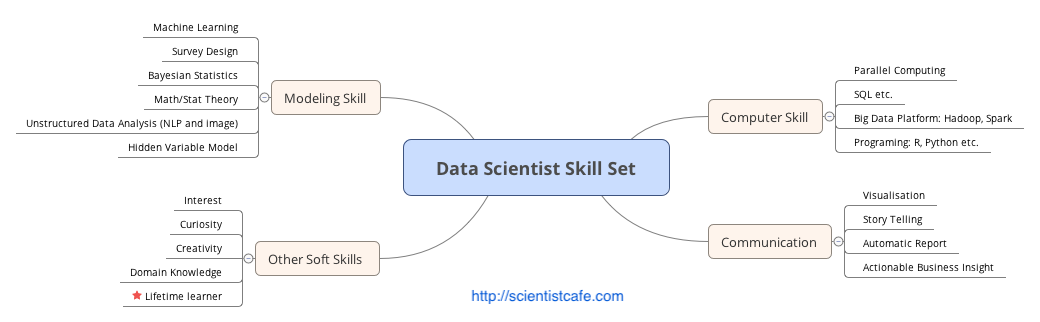
\includegraphics{images/SkillEN.png}
\caption{}
\end{figure}

\subsection{Types of Learning}\label{types-of-learning}

There are three broad groups of styles: supervised learning,
reinforcement learning, and unsupervised learning.

In supervised learning, each observation of the predictor measurement(s)
corresponds to a response measurement. There are two flavors of
supervised learning: regression and classification. In regression, the
response is a real number such as the total net sales in 2017, or the
yield of corn next year. The goal is to approximate the response
measurement as much as possible. In classification, the response is a
class label, such as dichotomous response such as yes/no. The response
can also have more than two categories, such as four segments of
customers. A supervised learning model is a function that maps some
input variables with corresponding parameters to a response y. Modeling
tuning is to adjust the value of parameters to make the mapping fit the
given response. In other words, it is to minimize the discrepancy
between given response and the model output. When the response y is a
real value, it is intuitive to define discrepancy as the squared
difference between model output and given the response. When y is
categorical, there are other ways to measure the difference, such as AUC
or information gain.

In reinforcement learning, the correct input/output pairs are not
present. The model will learn from a sequence of actions and select the
action maximizing the expected sum of the future rewards. There is a
discount factor that makes future rewards less valuable than current
rewards. Reinforcement learning is difficult for the following reasons:

\begin{enumerate}
\def\labelenumi{(\arabic{enumi})}
\item
  The rewards are not instant. If the action sequence is long, it is
  hard to know which action was wrong.
\item
  The rewards are occasional. Each reward does not supply much
  information, so its impact of parameter change is limited. Typically,
  it is not likely to learn a large number of parameters using
  reinforcement learning. However, it is possible for supervised and
  unsupervised learning. The number of parameters in reinforcement
  learning usually range from dozens to maybe 1,000, but not millions.
\end{enumerate}

In unsupervised learning, there is no response variable. For a long
time, the machine learning community overlooked unsupervised learning
except for one called clustering. Moreover, many researchers thought
that clustering was the only form of unsupervised learning. One reason
is that it is hard to define the goal of unsupervised learning
explicitly. Unsupervised learning can be used to do the following:

\begin{enumerate}
\def\labelenumi{(\arabic{enumi})}
\item
  Identify a good internal representation or pattern of the input that
  is useful for subsequent supervised or reinforcement learning, such as
  finding clusters.
\item
  It is a dimension reduction tool that is to provide compact, low
  dimensional representations of the input, such as factor analysis.
\item
  Provide a reduced number of uncorrelated learned features from
  original variables, such as principle component regression.
\end{enumerate}

\begin{figure}[htbp]
\centering
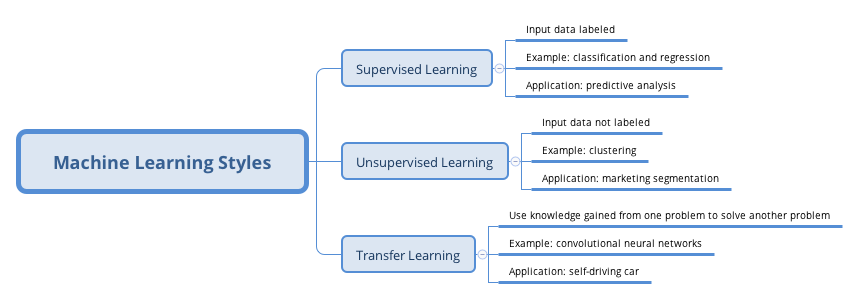
\includegraphics{images/LearningStyles.png}
\caption{}
\end{figure}

\subsection{Types of Algorithm}\label{types-of-algorithm}

The summary of various algorithms for data science in this section is
based on Jason Brownlee's blog ``(A Tour of Machine Learning
Algorithms){[}\url{http://machinelearningmastery.com/a-tour-of-machine-learning-algorithms/}{]}.''
We added and subtracted some algorithms in each category and gave
additional comments. The categorization here is based on the structure
(such as tree model, Regularization Methods) or type of question to
answer (such as regression). It is far less than perfect but will help
to show a bigger map of different algorithms. Some can be legitimately
classified into multiple categories, such as support vector machine
(SVM) can be a classifier, and can also be used for regression. So you
may see other ways of grouping. Also, the following summary does not
list all the existing algorithms (there are just too many).

\begin{enumerate}
\def\labelenumi{\arabic{enumi}.}
\tightlist
\item
  Regression
\end{enumerate}

Regression can refer to the algorithm or a particular type of problem.
It is supervised learning. Regression is one of the oldest and most
widely used statistical models. It is often called the statistical
machine learning method. Standard regression models are:

\begin{itemize}
\tightlist
\item
  Ordinary Least Squares Regression
\item
  Logistic Regression
\item
  Multivariate Adaptive Regression Splines (MARS)
\item
  Locally Estimated Scatterplot Smoothing (LOESS)
\end{itemize}

The least squares regression and logistic regression are traditional
statistical models. Both of them are highly interpretable. MARS is
similar to neural networks and partial least squares (PLS) in the
respect that they all use surrogate features instead of original
predictors.

They differ in how to create the surrogate features. PLS and neural
networks use linear combinations of the original predictors as surrogate
features \footnote{To be clear on neural networks, the linear
  combinations of predictors are put through non-linear activation
  functions, deeper neural networks have many layers of non-linear
  transformation}. MARS creates two contrasted versions of a predictor
by a truncation point. And LOESS is a non-parametric model, usually only
used in visualization.

\begin{enumerate}
\def\labelenumi{\arabic{enumi}.}
\setcounter{enumi}{1}
\tightlist
\item
  Similarity-based Algorithms
\end{enumerate}

This type of model is based on a similarity measure. There are three
main steps: (1) compare the new sample with the existing ones; (2)
search for the closest sample; (3) and let the response of the nearest
sample be used as the prediction.

\begin{itemize}
\tightlist
\item
  K-Nearest Neighbour {[}KNN{]}
\item
  Learning Vector Quantization {[}LVQ{]}
\item
  Self-Organizing Map {[}SOM{]}
\end{itemize}

The biggest advantage of this type of model is that they are intuitive.
K-Nearest Neighbour is generally the most popular algorithm in this set.
The other two are less common. The key to similarity based algorithms is
to find an appropriate distance metric for your data.

\begin{enumerate}
\def\labelenumi{\arabic{enumi}.}
\setcounter{enumi}{2}
\tightlist
\item
  Feature Selection Algorithms
\end{enumerate}

The primary purpose of feature selection is to exclude non-information
or redundant variables and also reduce dimension. Although it is
possible that all the independent variables are significant for
explaining the response. But more often, the response is only related to
a portion of the predictors. We will expand the feature selection in
detail later.

\begin{itemize}
\tightlist
\item
  Filter method
\item
  Wrapper method
\item
  Embedded method
\end{itemize}

Filter method focuses on the relationship between a single feature and a
target variable. It evaluates each feature (or an independent variable)
before modeling and selects ``important'' variables.

Wrapper method removes the variable according to particular law and
finds the feature combination that optimizes the model fitting by
evaluating a set of feature combinations. In essence, it is a searching
algorithm.

Embedding method is part of the machine learning model. Some model has
built-in variable selection function such as lasso, and decision tree.

\begin{enumerate}
\def\labelenumi{\arabic{enumi}.}
\setcounter{enumi}{3}
\tightlist
\item
  Regularization Method
\end{enumerate}

This method itself is not a complete model, but rather an add-on to
other models (such as regression models). It appends a penalty function
on the criteria used by the original model to estimate the variables
(such as likelihood function or sum of squared error). In this way, it
penalizes model complexity and contracts the model parameters. That is
why people call them ``shrinkage method.'' This approach is advantageous
in practice.

\begin{itemize}
\tightlist
\item
  Ridge Regression
\item
  Least Absolute Shrinkage and Selection Operator (LASSO)
\item
  Elastic Net
\end{itemize}

\begin{enumerate}
\def\labelenumi{\arabic{enumi}.}
\setcounter{enumi}{4}
\tightlist
\item
  Decision Tree
\end{enumerate}

Decision trees are no doubt one of the most popular machine learning
algorithms. Thanks to all kinds of software, implementation is a no
brainer which requires nearly zero understanding of the mechanism. The
followings are some of the common trees:

\begin{itemize}
\tightlist
\item
  Classification and Regression Tree (CART)
\item
  Iterative Dichotomiser 3 (ID3)
\item
  C4.5
\item
  Random Forest
\item
  Gradient Boosting Machines (GBM)
\end{itemize}

\begin{enumerate}
\def\labelenumi{\arabic{enumi}.}
\setcounter{enumi}{5}
\tightlist
\item
  Bayesian Models
\end{enumerate}

People usually confuse Bayes theorem with Bayesian models. Bayes theorem
is an implication of probability theory which gives Bayesian data
analysis its name.

\[Pr(\theta|y)=\frac{Pr(y|\theta)Pr(\theta)}{Pr(y)}\]

The actual Bayesian model is not identical to Bayes theorem. Given a
likelihood, parameters to estimate, and a prior for each parameter, a
Bayesian model treats the estimates as a purely logical consequence of
those assumptions. The resulting estimates are the posterior
distribution which is the relative plausibility of different parameter
values, conditional on the observations. The Bayesian model here is not
strictly in the sense of Bayesian but rather model using Bayes theorem.

\begin{itemize}
\tightlist
\item
  Naïve Bayes
\item
  Averaged One-Dependence Estimators (AODE)
\item
  Bayesian Belief Network (BBN)
\end{itemize}

\begin{enumerate}
\def\labelenumi{\arabic{enumi}.}
\setcounter{enumi}{6}
\tightlist
\item
  Kernel Methods
\end{enumerate}

The most common kernel method is the support vector machine (SVM). This
type of algorithm maps the input data to a higher order vector space
where classification or regression problems are easier to solve.

\begin{itemize}
\tightlist
\item
  Support Vector Machine (SVM)
\item
  Radial Basis Function (RBF)
\item
  Linear Discriminate Analysis (LDA)
\end{itemize}

\begin{enumerate}
\def\labelenumi{\arabic{enumi}.}
\setcounter{enumi}{7}
\tightlist
\item
  Clustering Methods
\end{enumerate}

Like regression, when people mention clustering, sometimes they mean a
class of problems, sometimes a class of algorithms. The clustering
algorithm usually clusters similar samples to categories in a centroidal
or hierarchical manner. The two are the most common clustering methods:

\begin{itemize}
\tightlist
\item
  K-Means
\item
  Hierarchical Clustering
\end{itemize}

\begin{enumerate}
\def\labelenumi{\arabic{enumi}.}
\setcounter{enumi}{8}
\tightlist
\item
  Association Rule
\end{enumerate}

The basic idea of an association rule is: when events occur together
more often than one would expect from their individual rates of
occurrence, such co- occurrence is an interesting pattern. The most used
algorithms are:

\begin{itemize}
\tightlist
\item
  Apriori algorithm
\item
  Eclat algorithm
\end{itemize}

\begin{enumerate}
\def\labelenumi{\arabic{enumi}.}
\setcounter{enumi}{9}
\tightlist
\item
  Artificial Neural Network
\end{enumerate}

The term neural network has evolved to encompass a repertoire of models
and learning methods. There has been lots of hype around the model
family making them seem magical and mysterious. A neural network is a
two-stage regression or classification model. The basic idea is that it
uses linear combinations of the original predictors as surrogate
features, and then the new features are put through non-linear
activation functions to get hidden units in the 2nd stage. When there
are multiple hidden layers, it is called deep learning, another over
hyped term. Among varieties of neural network models, the most widely
used ``vanilla'' net is the single hidden layer back-propagation
network.

\begin{itemize}
\tightlist
\item
  Perceptron Neural Network
\item
  Back Propagation
\item
  Hopield Network
\item
  Self-Organizing Map (SOM)
\item
  Learning Vector Quantization (LVQ)
\end{itemize}

\begin{enumerate}
\def\labelenumi{\arabic{enumi}.}
\setcounter{enumi}{10}
\tightlist
\item
  Deep Learning
\end{enumerate}

The name is a little misleading. As mentioned before, it is multilayer
neural network. It is hyped tremendously especially after AlphaGO
defeated Li Shishi at the board game Go. We don't have too much
experience with the application of deep learning and are not in the
right position to talk more about it. Here are some of the common
algorithms:

\begin{itemize}
\tightlist
\item
  Restricted Boltzmann Machine (RBN)
\item
  Deep Belief Networks (DBN)
\item
  Convolutional Network
\item
  Stacked Autoencoders
\item
  Long short-term memory (LSTM)
\end{itemize}

\begin{enumerate}
\def\labelenumi{\arabic{enumi}.}
\setcounter{enumi}{11}
\tightlist
\item
  Dimensionality Reduction
\end{enumerate}

Its purpose is to construct new features that have significant physical
or statistical characteristics, such as capturing as much of the
variance as possible.

\begin{itemize}
\tightlist
\item
  Principle Component Analysis (PCA)
\item
  Partial Least Square Regression (PLS)
\item
  Multi-Dimensional Scaling (MDS)
\item
  Exploratory Factor Analysis (EFA)
\end{itemize}

PCA attempts to find uncorrelated linear combinations of original
variables that can explain the variance to the greatest extent possible.
EFA also tries to explain as much variance as possible in a lower
dimension. MDS maps the observed similarity to a low dimension, such as
a two-dimensional plane. Instead of extracting underlying components or
latent factors, MDS attempts to find a lower-dimensional map that best
preserves all the observed similarities between items. So it needs to
define a similarity measure as in clustering methods.

\begin{enumerate}
\def\labelenumi{\arabic{enumi}.}
\setcounter{enumi}{12}
\tightlist
\item
  Ensemble Methods
\end{enumerate}

Ensemble method made its debut in the 1990s. The idea is to build a
prediction model by combining the strengths of a collection of simpler
base models. Bagging, originally proposed by Leo Breiman, is one of the
earliest ensemble methods. After that, people developed Random Forest
\citep{Ho1998, amit1997} and Boosting method
\citep{Valiant1984, KV1989}. This is a class of powerful and effective
algorithms.

\begin{itemize}
\tightlist
\item
  Bootstrapped Aggregation (Bagging)
\item
  Random Forest
\item
  Gradient Boosting Machine (GBM)
\end{itemize}

\begin{figure}[htbp]
\centering
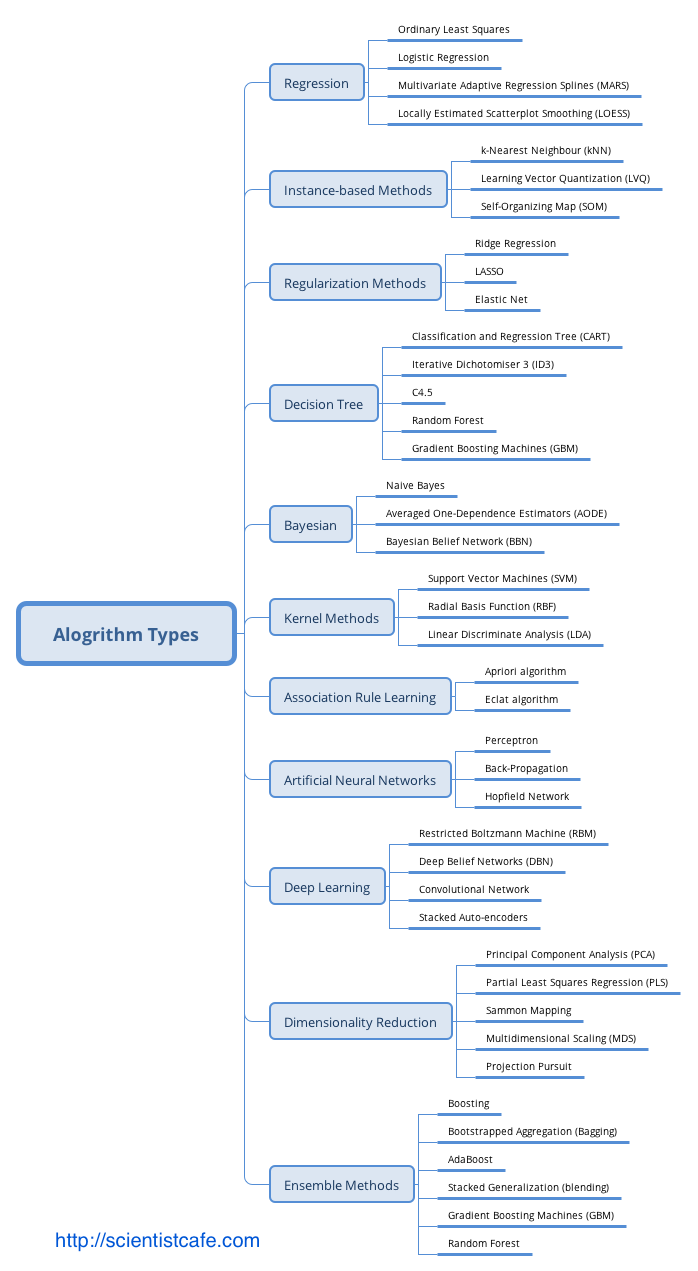
\includegraphics{images/AlogrithmTypes.png}
\caption{}
\end{figure}

\section{References}\label{references}

\bibliography{bibliography.bib}

\backmatter
\printindex

\end{document}
